\begin{mybilan}
	\twoCol{
	\begin{itemize}
		\item Un objet diffusant ne peut être vu que \kw{s'il est éclairé}.
		\item La lumière diffusée par un objet peut entrer dans l'\oe il d'un observateur si \kw{aucun obstacle opaque} n'est placé entre cet objet et l'\oe il de l'observateur.
		\item Pour voir un objet, la lumière émise par cet objet doit arriver dans les yeux de la personne qui l'observe.
	\end{itemize}

	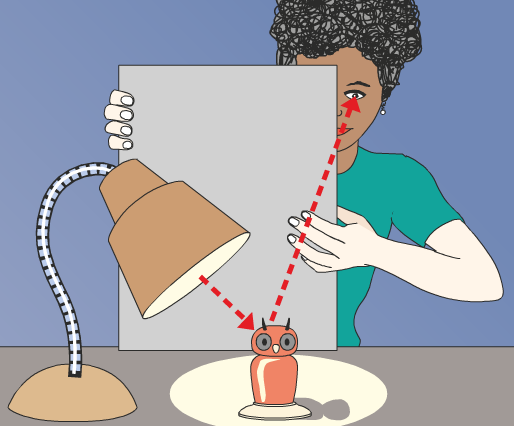
\includegraphics[scale=0.6]{bilan2}
}
\end{mybilan}